\documentclass{llncs}
\usepackage{times}

\usepackage{a4}
\usepackage[utf8]{inputenc}
\usepackage[T1]{fontenc}
\usepackage{lmodern}
\usepackage{libertine}
%\usepackage{fontspec}

%\usepackage[margin=3cm,nohead]{geometry}
\usepackage{epstopdf}
\usepackage{graphicx}
\usepackage{fancyvrb}
\usepackage{amsmath}
\usepackage[backend=biber]{biblatex}
\addbibresource{references.bib}
%\renewcommand{\baselinestretch}{1.5}

\begin{document}
\mainmatter
\title{Uma pesquisa sobre Software Defined Networking}

\titlerunning{Pesquisa sobre SDN}

\author{Miguel Cruz \and Dinis Peixoto \and João Tomás}

\authorrunning{Miguel \and Dinis \and Tomas}

\institute{
University of Minho, Department of  Informatics, 4710-057 Braga, Portugal\\
e-mail: \{a108574, a108566, a108656\}@alunos.uminho.pt
}

\date{}

\maketitle
\begin{abstract}
\textit{Software Defined Network} (SDN) é uma abordagem de redes,que surge em resposta ao crescimento explonencial das \textit{information and communication technologies} (ICT), que visa simplificar a sua gestão e permitir a inovação através de redes 
dinâmicas e programáveis, que estabelecem um contraponto face às arquiteturas estáticas das redes tradicionais, descentralizadas e complexas. De facto, o objetivo do SDN é melhorar o controlo da rede, permitindo que as empresas e os fornecedores de serviço respondam
rapidamente às mudanças nos requisitos dos negócios, possibilitando que um administrador molde o tráfego a partir de um terminal de controlo centralizado sem recorrer a switches individuais. Conseguindo alterar as condições de qualquer switch de rede necessário - priorizando ou inibindo (parcialmente/totalmente) pacotes específicos de forma granular. 
Isto é particularmente útil em arquiteturas \textit{multi-tenant} em nuvem, uma vez que permite que administradores giram o tráfego de forma flexível e mais eficiente. 
Neste trabalho apresentamos uma definição de SDN e a sua arquitetura, bem como os seus principais benefícios, mas também os seus maiores desafios. Aliado a isto, faremos uma alusão às redes híbridas, bem como o desempenho em larga escala. E para concluir uma sucinta conclusão sobre o trabalho.
\end{abstract}

\section{Introdução}

\paragraph{} O crescimento exponencial das *\textit {information and communication technologies} (ICT), particularmente, \textit {cloud computing}, a automação de redes e as redes de \textit {data centers}, é catalisada pela integração de sistemas baseados no SDN. \cite{paper1}
 Com a globalização do digital e o aumento do volume de dispositivos conectados, as arquiteturas de redes tradicionais descentralizadas, que dependem de \textit {hardware} especializado, revelaram-se ineficientes face à necessidade de flexibilidade e de escalabilidade. 
 Neste medida, as redes tradicionais oferecem pouca flexibilidade na gestão do tráfego, bem como incapacidade na resposta às novas exigências computacionais, tais como a baixa latência ou a segmentação de rede. 
 Em contraste, o SDN é uma abordagem inovadora que visa simplificar o tráfego através de redes dinâmicas e programáveis. 
 Com a centralização via \textit {software}, os administradores podem moldar as condições da rede conforme a necessidade, otimizando a utilização de recursos, bem como melhorando a qualidade de serviço (QoS).
 \paragraph{}
Complementarmente, o SDN define-se pelas seguintes características. Primeiramente, a capacidade de desassociar o plano de dados do plano de controlo. \cite{paper3}
 Em segundo lugar, o SDN possui um plano de controlo indefinido, o que permite que seja controlado por um único \textit {software}.
 Por conseguinte, o plano de controlo do SDN estende o seu controlo sobre os elementos do plano de dados da rede, por meio do OpenFlow, programa de interface mais utilizado mundialmente.
 Paralelamente, a arquitetura do SDN providencia que um administrador visione a rede globalmente, mas também que faça alterações globalmente.
 \paragraph{}
Neste trabalho, procuramos apresentar a definição de SDN, bem como a sua arquitetura, aliada aos desenvolvimentos existente à data do SDN, bem como abordagens que visionem o desenvolvimento do SDN.
 O trabalho está organizado da seguinte forma. Na segunda secção, apresentaremos uma definição de SDN, a par dos seus benefícios  e principais desafios.
 Nas duas secções seguintes, apontaremos prospecções de futuros desenvolvimentos possíveis do SDN. 
 Particularmente, na secção três indicaremos um sistema híbrido do SDN e as \textit {legacy networks}, e a secção quatro exibe o desempenho do SDN em larga escala, bem como a sua prospecção face às otimizações mencionadas anteriormente. 
 E, uma sucinta conclusão, que engloba o as implementações atuais do SDN, mas também uma antevisão das implementações futuras, e dos seus benefícios, na secção seis.
 \paragraph{}
\section{SDN: definição, benefícios e desafios}
\paragraph{}
Devido à sua emergência, o SDN ainda não dispõe uma definição consensual.
Nesta secção, iremos primeiramente apresentar a mais definição mais creditada, e posteriormente, os benefícios do SDN.

\subsection{Definição de SDN}
\paragraph{}
De acordo com a Open Networking Foundation (ONF), \textit{Software Defined Networking} (SDN) é uma arquitetura de redes dinámica, controlável, econômica e flexível, tornando-a ideal para os usos de banda larga das aplicações atuais. 
Esta arquitetura desassocia as funções de controlo e encaminhamento da rede, possiblitando que o controlo da rede seja diretamente programável. \cite{fundation2012software}
\paragraph{}
Convergentemente, o ONF disp\~{o}e de um modelo de refer\~{e}ncia do SDN, como ilustrado na figura \ref{fig:architecture}
\begin{figure}
\begin{center}
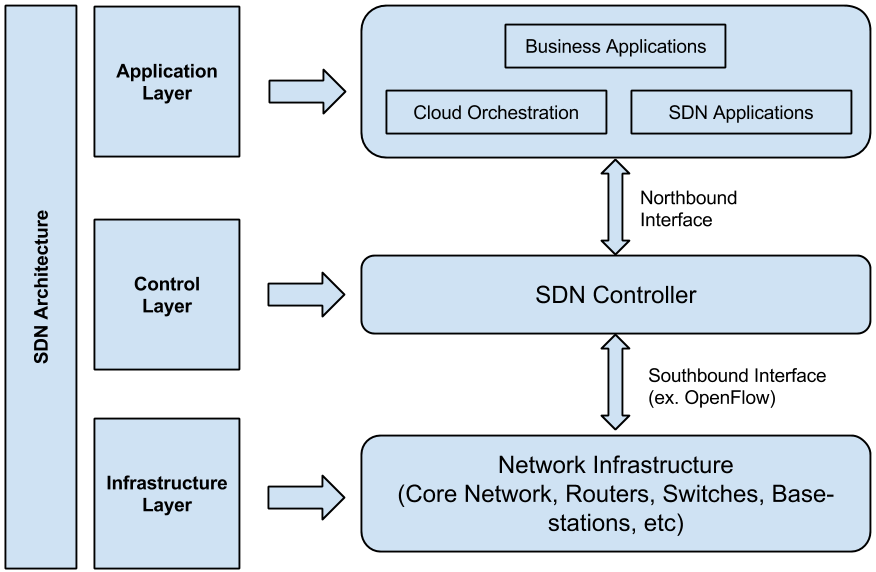
\includegraphics[scale=0.40]{figura1.png}
\caption{Modelo de Referência do SDN, segundo a ONF.}
\label{fig:architecture}
\end{center}
\end{figure} 
\paragraph{}

A camada de infraestrutura consiste em dispositivos de comutação (por exemplo, \textit{switches}, \textit{routers}, etc.) no plano de dados.
As funções destes dispositivos de comutação são basicamente duplas. 
Primeiro, são responsáveis por recolher o estado da rede, armazená-los temporariamente em dispositivos locais e enviá-los para os controladores. 
O estado da rede pode incluir informações como a topologia da rede, estatísticas de tráfego e utilizações da rede. 
Em segundo lugar, são responsáveis pelo processamento de pacotes com base em regras fornecidas por um controlador.
\paragraph{}
A camada de controlo faz a ponte entre a camada de aplicação e a camada de infraestrutura, através das suas duas interfaces. Para a interação descendente com a camada de infraestrutura (ou seja, a interface virada a sul), especifica funções para os controladores acederem a funções fornecidas pelos dispositivos de comutação. As funções podem incluir relatórios do estado da rede e importação de regras de encaminhamento de pacotes. Para uma interação ascendente com a camada de aplicação (ou seja, a interface norte), fornece pontos de acesso de serviço em várias formas, por exemplo, uma \textit{Application Programming Interface} (API). As aplicações SDN podem aceder a informações de estado de rede reportadas a partir de dispositivos de comutação através desta API, tomar decisões de ajuste do sistema com base nessas informações e executar essas decisões configurando regras de encaminhamento de pacotes para dispositivos de comutação utilizando esta API. Como existirão múltiplos controladores para um grande domínio administrativo de rede, uma interface de comunicação “leste-oeste” entre controladores também exigirá que os controladores partilhem informações de rede e coordenem os seus processos de tomada de decisão.
\paragraph{}
A camada de aplicação contém aplicações SDN concebidas para satisfazer os requisitos do utilizador. Através da plataforma programável fornecida pela camada de controlo, as aplicações SDN são capazes de aceder e controlar dispositivos de comutação na camada de infraestrutura. Exemplos de aplicações SDN podem incluir o controlo de acesso dinâmico, o balanceamento de carga do servidor e a virtualização de rede.

\subsection{Benefícios do SDN}
\paragraph{}
O SDN tem por característica a capacidade de desassociar o plano de controlo do plano de dados. Esta característica poderá resultar em inúmeros benefícios a nível da 
configuração, otimização, performance e inovação nos sistemas de redes. Como se averigua na figura \ref{fig:tabela}
\paragraph{}
\begin{figure}
\begin{center}
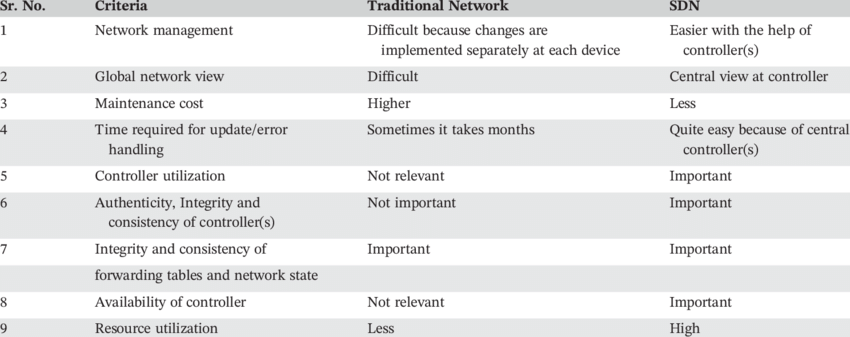
\includegraphics[scale=0.40]{tabela.png} 
\end{center}
\caption{Tabela Comparativa entre o SDN e redes tradionais.}
\label{fig:tabela}
\end{figure} 
\paragraph{}
Na gestão de redes a configuração representa um ponto fulcral, particularmente, quando um novo dispositivo é conectado a uma rede previamente existente, uma configuração
devida é necessária para obter uma operação de redes estável. O modelo contemporâneo de redes ainda apresenta um grande desafio na configuração automática e dinâmica de redes.
Em contra ponto, o SDN solucionará este problema, a unificação do plano de controlo sobre os dispositivos de redes, como \textit{switches}, \textit{routers} e a \textit{firewall},
permite configurar dispositivos de rede a partir de um único ponto, via software. Assim, uma rede pode ser configurada programaticamente e dinamicamente com base no \textit{status} da rede. \cite{paper1}
\paragraph{}
Nas operações de redes um dos objetivos é maximizar a utilização da infrastutura da rede. Contudo, as abordagens atuais procuram a otimização de subconjunto de redes, ou,
na qualidade de experiência dos usuários nos serviços de redes. Estas abordagens podem resultar num descrescimo do desempenho, ou até, em conflitos entre operações de redes. 
O SDN permite um controlo centralizado com uma visão global e um controlo das informações entre as várias camadas da arquitetura da rede. Complementarmente, os desafios contemporâneos
de otimização seriam resolvidos com algoritmos centralizados adequados.
\paragraph{}
A continua evolução de redes deverá encorajar a inovação das aplicações de redes, ao ínves de tentar prever com precisão aplicações futuras. Assim, alta configurabilidade do
SDN permite uma separação entre redes virtuais, o que permite a realização de testes em ambientes reais. Deste modo, o SDN encoraja a inovação, na medida em que providencia 
uma plataforma de redes programável para implementar, exprimentar, e lançar novas ideias, aliado a remuneramentos flexíveis e convinientes. \cite{paper1}
\subsection{Desafios do SDN}
\paragraph{}
O SDN é o pico das arquiteturas de redes, pelo que é uma tecnologia emergente tão reverente. 
Como o SDN é uma arquitetura centralizada no plano de controlo, a eficiência do controlador impacta diretamente a escalabilidade do SDN, 
que se revela determinante para o sucesso do ecossitema SDN. Nesta medida, estes problemas fundamentais ainda não apresentam soluções definitivas.\cite{performance}
\paragraph{}
O projeto OpenFlow patricionado pela ONF, que a apresenta a definição mais creditada do SDN, não é de forma alguma o único modelo de SDN e uma solução concisa. 
Complementarmente um textit{driver open-source} do OpenFlow ainda não está disponível para o desenvolvimento de controladores de SDN.Mas também, o desenvolvimento de aplicações de SDN está condicionado pela inexistência uma liguagem de alto nível. 
Convergentemente, um ecossistema saudável que combine fornecedores, desenvolvedores e consumidores ainda está para surgir. \cite{paper1} 
\paragraph{}
Ainda que o SDN seja uma invoção em sistema de redes, a trasição de sistemas de redes tradionais para o SDN revelou-se um processo trabalhoso e disruptivo. Assim, problemas correntes incluem
a inoperabilidade  do sistema SDN com dispositivos de textit{legacy networks}, o desempenho e privacidade do controlo centralizado, e a falta de suporte especializado, por meio de suporte técnico.
Deste modo, as implementações de SDN são na sua maioria limitadas a ambientes de teste para fins de pesquisa. Os protótipos do SDN não se demonstram estáveis o suficiente para oferecerem confiança, para serem implementados em contextos reais, o que limita a disposição das empresas de adotá-lo em largas escalas.\cite{paper1}

\section{Integração de SDN com \textit{legacy networks}}
\paragraph{}
Um problema do OpenFlow é a utilização de redes virtualizadas, que é uma ferramenta essencial para os ambientes de experimentação.
À semelhança da virtualização, procura melhorar a alocação de recursos permitindo aos operadores criar pontos de verificação para a sua rede antes de fazer alterações, e garante que os clientes concorrentes possam partilhar os mesmos equipamentos de forma controlada e isolada. 
Permite ainda que um conjunto de \textit{switches} seja partilhado entre múltiplas redes lógicas, cada uma com a mesma lógica de encaminhamento distinta e utilizando o mesmo plano de encaminhamento de \textit{hardware}, que são hoje as principais características dos ambientes \textit{Future Internet} (FI).
\paragraph{}
No entanto, hoje em dia tanto as instalações de experimentação de FI como as redes OpenFlow enfrentam um grande desafio: como podem integrar estes ambientes com ambientes de rede híbrida (i.e., OpenFlow e Legacy Network)? 
Inicialmente é necessário conceptualizar \textit{Legacy Networks}, são redes com equipamentos utilizados por não-OpenFlow (e.g. a actual rede Internet) ou tecnologias que não são suportadas pelo OpenFlow (e.g. tecnologias de circuitos Camada 1 e Camada 0). 
Alguns dos desafios das redes OpenFlow estão relacionados com a compatibilidade e os requisitos de integração com ambientes de \textit{legacy networks}.
\paragraph{}
Outra questão, o OpenFlow não é capaz de manipular ou gerir equipamentos de legado pelo protocolo OpenFlow e, como resultado, é extremamente difícil alocar recursos em \textit{legacy networks} para ligar dois ambientes OpenFlow. 
Para além de outros problemas que surgem durante a implementação, existe um problema prático que envolve \textit{ legacy switches} que não suportam o protocolo OpenFlow e precisam de ser substituídos ou atualizados.

\section{Desempenho em implementações em larga escala}
\paragraph{}
Podemos dizer que as tecnologias e protocolos habilitadas pelo SDN contribuem significativamente para o sucesso do \textit {cloud computing}, bem como para a automação de redes e \textit {data centers}. O SDN permite satisfazer os requirementos de recursos \textit{on demand} dos utilizadores na \textit{cloud}. 
É uma infraestrutura inovadora que consegue preencher a lacuna entre as redes convencionais de \textit{data centers} e os requesitos computacionais e de armazenamento dos utilizadores.
O SDN consegue superar as tecnologias de redes existentes, oferecendo serviços extra oferecendo vários serviços sem esforços extra e despesas gerais a um custo mínimo, como gestão de rede consolidada, segurança de rede robusta, escalabilidade, adaptabilidade, estratégias de \textit {backtesting} mais seguras, unificação perfeita de recursos de \textit{cloud} e entrega garantida de conteúdo.

\section{Conclusões}
\paragraph{}
Para concluir este trabalho, apresentaremos uma resumo sucinto dos temas centrais abordados.
\paragraph{}
O desenvolvimento dos ICT requer um acesso mais conveniente à internet em banda larga e gestão da rede de forma mais dinâmica, establecendo um contraponto com as redes tradicionais. 
Nesta medida, o SDN é considerado uma solução promissora. Neste trabalho, apresentamos a definição mais consensual de SDN, providenciada pela ONF, bem como os benefícios do SDN. 
Paralelamente, abordamos integração de \textit{legacy networks} com o SDN, isto é, a prospeção de redes híbridas. 
E, sequencialmente, a implementação do SDN em larga escala.
Mas também os principais desafios do SDN, como a padronização, implementação e a implantação.

\printbibliography

\end{document}